\documentclass[journal=jctcce,manuscript=article]{achemso}

\usepackage[version=3]{mhchem} % Formula subscripts using \ce{}
\usepackage[T1]{fontenc}       % Use modern font encodings
\usepackage{graphicx}
\usepackage[table,xcdraw]{xcolor}

\author{Nathan Lim}
\email{limn1@uci.edu}
\affiliation[University of California, Irvine]
{Department of Pharmaceutical Sciences}

\title{Sensitivity in predicted relative binding free energies from incremental ligand changes within a model binding site}

\begin{document}

\begin{abstract}
Despite innovations in sampling techniques for molecular dynamics (MD), reliable prediction of protein-ligand binding free energies from MD remains a challenging problem, even in well studied model binding sites like the apolar cavity of T4 Lysozyme L99A\cite{Boyce2009}.
In this study, we model recent experimental results that show the progressive opening of the binding pocket in response to a series of homologous ligands \cite{Merski2015}.
Even while using enhanced sampling techniques, we demonstrate that the predicted relative binding free energies (RBFE) are still highly sensitive to the initial protein conformational state.
Particularly, we highlight the importance of sufficient sampling of protein conformational changes and possible techniques for addressing the issue.
\end{abstract}

\pagebreak

%%%%WRITING TIPS%%%%%
%ALWAYS ACTIVE VOICE --> Direct, emphasize the performer of the action.
%"First sentence of each paragraph should tell the reader what you expect them to get out of the paragraph that follows"

%"Results should typically start with a paragraph describing your approach in broad terms"
%"Give them the conceptual tools to understand your work but not more"

%%%%%%%%%%%%%%%%%%%%%


\section{Introduction}
%Jotted down ideas only
Medicinal chemistry programs typically focus on changes in ligand binding affinity from incremental changes to the ligand.
Focus on how the protein adapts to the changes in the ligand is generally neglected.
T4 L99A is well studied experimentally and computationally.
It is frequently used as a model binding site in free energy prediction studies.
In this study, 8 congeneric ligands were investigated, where addition of a single methyl group was used to lengthen the ligand.
Through determination of protein-ligand bound x-ray crystal structures it was revealed T4 Lysozyme adopts 3 discrete conformations in response the series of growing ligands.
Consideration of the protein adaptations into discrete conformations may be an important aspect in inhibitor design.

\section{Results}
\subsection*{Dependence on protein starting conformation}
%P1: Open with the main problem in default protocol. 
%Describing the approach in broad terms. 
%Give them the conceptual tool to understand most of the work.
%Drive back the main problem in default protocol.
Using the default FEP/REST methodology\cite{FEP/REST}, we find calculated free energies significantly depend on the protein starting conformation, especially for large perturbations (i.e. opening the cavity from the closed state).
To illustrate this, we begin our molecular dynamics simulations both from the protein closed and open conformations then perform alchemical transformations to ligands that occupy the opposite protein conformational state.
In this study, root-mean-square-deviation (RMSD) of the backbone atoms in the F-helix is used to determine the conformational state of the protein over the course of the simulation.
Here, we demonstrate the default 5ns simulation time and REST region selection in the Schrodinger FEP workflow are insufficient for adequate sampling of the motion in the F-helix and does not eliminate the dependence on the initial protein state.

%P2: Discuss closed-open case to show the problem in default protocol
An examination of the largest alchemical transformation, benzene to n-hexylbenzene, highlights the sampling problems faced when using the standard FEP/REST protocol.
From experimental data of ligand occupancies (Table~\ref{tbl:loop-occ}), we expect in our simulations of n-hexylbenzene to see the protein primarily in the open state over the closed state.
Instead, we find the protein remains trapped in its initial conformational state whether we start from closed (Fig~\ref{fig:c_opls3_1/RMSD-replica11}) or open (Fig~\ref{fig:o_opls3_1/RMSD-replica11}) over the course of the 5ns simulation.
From the protein closed simulation, the protein only begins to enter the intermediate state around 3ns but never enters the open conformation.
As the protein tries to accommodate n-hexylbenzene and enter its preferred open state, protein-ligand strain results, yielding a positive value for $\Delta\Delta G_{calc}$(+4.13 kcal/mol).
On the other hand, in the protein open simulations, the protein already begins in its preferred state for n-hexylbenzene and stays only in this open state.
As expected, the $\Delta\Delta G_{calc}$ comes out negative(-0.61 kcal/mol) as there is no occurrence of large protein-ligand strain in order to open the cavity.
Ultimately, we arrive at two very different relative free energies values, where the discrepancy is as large as +4.74 kcal/mol for the same transformation of benzene to n-hexylbenzene\footnotemark.
Collectively, when we view the discrepancy of all calculations involving closed-open transformations we find the root-mean-square-error (RMSE) to be +4 kcal/mol (Table~\ref{tbl:C-O}).  
%DLM may need to say error relative to what (i.e. this is like the RMS discrepancy or something, right?) Maybe should use RMSD and mention on first use that it will be used to measure the RMS deviation between trials starting from open and those starting from closed, and use RMSE for RMS error relative to experiment (when needed).
Clearly, despite the use of FEP/REST, we are unable to adequately sample all the relevant states within the standard 5ns time frame, resulting in such large differences in $\Delta\Delta G_{calc}$.

\footnotetext{It should be noted that the binding affinities of n-pentyl/n-hexylbenzene to T4-L99A are not known and were inaccessible in experimental studies due to solubility limits. \cite{Merski2015}
For cases involving these ligands, we only focus on the convergence of the calculated free energies between simulations starting from protein closed or open.}

%P3: Discuss close-int case to show there is still a dependence even for small changes
In the case of more moderate alchemical transformations, such as cases that involve the set of closed ligands (i.e. benzene to n-propylbenzene) to intermediate ligands (i.e. sec-/n-butylbenzene), we find that the calculated free energies still have some (albeit much smaller) dependence on the initial protein conformation using the default protocol.
For the set of transformations to the intermediate state, the discrepancy RMSE in $\Delta\Delta G_{calc}$ for protein closed versus open simulations is +0.60 kcal/mol (Table~\ref{tbl:C-I}). 
However, when we compare $\Delta\Delta G_{calc}$ against $\Delta\Delta G_{exp}$ for transformations involving n-butylbenzene, we find that simulations starting from the protein closed conformation are further from converging to $\Delta\Delta G_{exp}$ than when starting from the protein open conformation.
From the protein closed simulations, the RMSE from $\Delta\Delta G_{exp}$ is +1.40 kcal/mol (Table~\ref{tbl:C-nbutyl_closed}) while the protein open simulations have a RMSE of +0.70 kcal/mol (Table~\ref{tbl:C-nbutyl_open}).
Based on experimental evidence (Table~\ref{tbl:loop-occ}), we should expect to see some sampling (~30\%) of the open conformation for the n-butylbenzene ligand if the calculations are converged.
Evidently, we find the simulations remain trapped in their respective starting conformations, resulting in inadequate sampling in the protein closed simulations (Fig.~\ref{fig:c_exp_opls3_11/RMSD-replica11}) versus the protein open simulations (Fig.~\ref{fig:o_exp_opls3_24/RMSD-replica11}).
Despite performing much smaller alchemical transformations, we still encounter sampling problems that result in $\Delta\Delta G_{calc}$ that depend on the intial protein conformation, evident when comparing to $\Delta\Delta G_{exp}$.

\subsection*{REST improvements (pREST)}
%P1: Recap problem, summarize solution and its effect
Primarily, we encounter major sampling problems when we begin our simulations from the protein closed state and attempt a mutation which should result in the helix opening.
In order to facilitate protein motion, we included 3 key residues spanning the F-helix region into the REST region, which we will denote simulations using this with pREST. %(see Methods for details?)
By expanding the REST region, we are able to drive the F-helix out its initial state trap faster by locally heating up key regions and thereby reduce our problem with inadequate sampling.

%P2 REST improvement qualitatively
To demonstrate the REST improvement over the default protocol, we return to the case of benzene to n-hexylbenzene.
Here, we show the facilitation of the helix motion by first referring to Fig~\ref{fig:c_opls3_1/RMSD-replica11} which shows that there is no sampling of the open state for the default protocol.
On the other hand with the pREST, we see a few open state points around 3ns and even a single open point before closing again in our initial step. (Fig~\ref{fig:c_opls3_rest1_1/RMSD-replica11}.
Alternatively, we can further illustrate the enhancement of protein transitions by viewing all replicas collectively. 
In Fig~\ref{fig:c_opls3_1/colormap} and Fig~\ref{fig:c_opls3_rest1_1/colormap}, we perform the same RMSD analysis but instead represent each time point as a colored bar and no longer plot the raw RMSD.
Visually, it is easy to see that there are far less transitions in default simulations (Fig~\ref{fig:c_opls3_1/colormap}) as opposed to pREST simulations (Fig~\ref{fig:c_opls3_rest1_1/colormap}).
%DLM: Nice graphs! Will need axis/color labels though. But these are very helpful.
 
%P3 REST improvement quantitatively in C-O and C-I sets
Collectively, for all our closed/open and closed/intermediate transformations using pREST, we find only some minor improvements in the discrepancy RMSE and even cases where we perform worse.
For closed/open transformations (Table~\ref{tbl:C-O_pREST}), the discrepancy RMSE improves to +2.78 kcal/mol (previously +4 kcal/mol) but gets regresses slightly to +0.78 kcal/mol (previously +0.60 kcal/mol) for closed/intermediate cases (Table~\ref{tbl:C-I_pREST}).
In general, simulations starting from the closed state had $\Delta\Delta G_{calc}$ values that moved towards favorability (i.e. more negative $\Delta\Delta G_{calc}$) and while protein open simulations $\Delta\Delta G_{calc}$ values tended towards unfavorability (i.e. more positive $\Delta\Delta G_{calc}$).
This is indicative of the fact that pREST is indeed improving sampling, but it is evident that our $\Delta\Delta G_{calc}$ are far from convergence given the discrepancy RMSE is still large, especially for closed/open transformations.

\subsection*{Longer pREST simulations}
%P1 Recap problem, summarize solution and effect
Although we see improvements in sampling with pREST, the standard implemented time frame of 5ns clearly is not long enough completely capture the transition of closed to open in the helix.
Here, we simulate 55ns for closed/open transformations and take the final 15ns of the simulation while for closed/intermediate we simulate 25ns and take the last 10ns of the simulation, discarding the initial time as additional equilibration time. %DLM: SOmewhere - not necessarily here - you'll want to explain why these choices for times were made. 
In simply running longer, we allow our simulations to perform more exchanges across replicas and thereby allow for better sampling of all conformational states.

%P2 Longer simulation improvements qualitatively
Returning to our most extreme transformation, benzene to n-hexylbenzene, we have shown pREST alone does not allow for adequate sampling of the open state (Fig~\ref{fig:c_opls3_rest1_1/RMSD-replica11}).
Now, when we run much longer we see far more frequent transitions between all the protein conformational states in the final 10ns window (Fig~\ref{fig:c_opls3_rest1_1/45-55ns/RMSD-replica11}).
In viewing all the replicas (Fig~\ref{fig:c_opls3_rest1_1/cmap-45-55ns}), we illustrate the dramatic increase in protein conformational sampling in stark contrast to our 5ns simulations (Fig~\ref{fig:c_opls3_rest1_1/colormap}). 
%DLM: If I were reviewing this I would ask if it's really that the transitions are more frequent, or if it's that you have the other protein conformation present in some replicas (lambda values) and it is walking between lambda values. That is to say, do you actually see the protein transitioning more often, or do you just see more frequent appearance of the open conformation in simulations? (This can be deconvoluted rigorously, it turns out; we may want to talk about this aspect.) 

%P3 Longer simulation improvements quantitatively
By simulating longer with pREST we dramatically increase our sampling of the intermediate/open states and almost entirely eliminate the dependence on the initial protein conformational state.
For the set of closed/open transformations the discrepancy RMSE dramatically falls to +0.57 kcal/mol (Table ~\ref{tbl:C-O_pREST-40-55ns}).
In the set of closed/intermediate transformations, only a few cases required an extended simulation time of 25ns, after doing so we obtain an overall RMSE of +0.42 kcal/mol (Table ~\ref{tbl:C-I_pRESText}). 
There still remains some discrepancy between $\Delta\Delta G_{calc}$ from protein open or closed simulations, but it now falls within a much more reasonable range of less than +1 kcal/mol. 
 
\section{Discussion}
%%%%TIPS%%%%
%"Discussion section should be constructed like a normal pyramid, stating your most specific research conclusions before broadening out to encompass wider ideas"
%"Lead your readers through an overview that describes how your results fit into the bigger picture"
%Discussion section should be able to somewhat stand on its own so readers do not have to constantly reference results section.

%P1: Restate problem: Convergence issues from protein conformational changes
%Even small rearrangements present sampling challenges which impact FE accuracy
%Magnitude/Impact of initial protein conformation
In this study, we find that relative free energy calculations can suffer from substantial convergence problems resulting from relatively modest protein conformational changes.
Although, the protein conformational changes in T4 lysozyme (L99A) are extremely localized to a rearrangement of a single helix, we still encounter sampling challenges.
These problems have profound implications for the accuracy of computed relative free energies in these cases.
Particularly, we find that calculated relative free energies can depend on the initial protein conformational state by up to 4 kcal/mol.

%P2: Restate the experiment carried out to remind the reader.
%Remind main analysis technique and the main idea we can draw from it
By looking at cases that involve a conformation change in the protein, we show the $\Delta\Delta G_{calc}$ is sensitive to the initial protein conformational state.
Such cases are when the alchemical transformation involves mutating ligands that primarily occupy the closed state (i.e. benzene to n-propyl) into ligands that occupy the intermediate (i.e. sec-/n-butyl) or open states (n-pentyl/n-hexyl) (Table~\ref{tbl:loop-occ}).
In tracking the RMSD relative to the crystallographic protein closed structure, we show the protein remains trapped in its initial state throughout the simulation when using the implemented default protocol.
Through remaining trapped, we are unable to adequately sample the correct protein-ligand conformational states and thereby poorly computed $\Delta\Delta G_{calc}$. 

%P3: Broader implications of this study
%Restate general trends from protein closed vs open
%Explicitly state the implications
Without prior knowledge of preferred protein conformational states on ligand binding, we can arrive at very different binding affinity predictions that are sensitive to the initial protein state.
Generally, from protein closed simulations we found $\Delta\Delta G_{calc}$ were highly positive and unfavorable, a result from strain in the protein as the ligand begins to grow in the binding cavity.
However, in protein open simulations we tended to see $\Delta\Delta G_{calc}$ that were negative and favorable as no protein-ligand strain is encountered (Table~\ref{tbl:C-O}).
If we only had the crystal structure of the closed protein-ligand complexes, we would blindly conclude that the much larger, open ligands bind worse than smaller ones.
On the other hand, if only the open protein-ligand complexes were available, the opposite would be concluded in that larger ligands are better binders than smaller ligands.

%P4: Restate the improvements from pREST
%Show where the improvement stems from
%Drive home main point again.
By including key residues into the REST region and simulating longer, we reduce the $\Delta\Delta G_{calc}$ dependence on the initial protein conformation to a more reasonable range of less than 1 kcal/mol.
Through expanding the REST region, intermediate lambda windows are able to more easily access the intermediate and open conformations by effectively heating key residues that would facilitate protein motion, illustrated in Fig~\ref{fig:c_opls3_rest1_1/colormap}.
Further, by simulating longer we allow for more exchanges between replicas, which in turn enhances sampling at our physically relevant end state lambda windows (Fig~\ref{fig:c_opls3_rest1_1/cmap-45-55ns}).   
With these modifications to the default protocol, we almost completely converge our $\Delta\Delta G_{calc}$ to the same value regardless of the starting protein conformation.

\section{Conclusions}
%P1: Broadly state the importance of knowing the various protein conformational states
Overall, we have shown that identification of discrete protein conformational states upon ligand binding is an essential factor to consider in inhibitor design.
Had we not known of the various protein-ligand states, our predictions would largely depend on the availability of known bound protein-ligand structures to start our simulations from.
Even more limiting, would be the case of only having the apo protein structure available, such as common in early drug discovery phases for new therapeutic targets.
Dangerously, a medicinal chemist can dock a library of ligands and run free energy predictions where the chemist would then discard ligands with "low" binding affinities.
Without prior knowledge of the existence of other protein conformational states, one would never know their calculations are actually incorrect. 

%P2: Broadly state the problem of protein sampling, how we resolved it, and the importance of this study.
Although FEP calculations have shown tremendous recent successes \cite{FEPplus}, we are still faced with challenges in adequate protein sampling.
Using T4 lysozyme (L99A) as our simple model system, we highlight sampling problems even from a relatively small (~1-3\AA) and localized single helix rearrangement in response to a growing ligand series.
In this study, we show only including ligand atoms into the REST region and using the typical 5ns simulation time leads to free energies that significantly depend on the initial protein conformational state. 
Only by expansion of the REST region to include key protein residues and longer simulation times were we able to eliminate the starting conformation dependence and come close to complete convergence.
More importantly, this demonstrates that special attention and care should be exercised in binding affinity predictions where regions of flexibility surround the binding site.

\section{Methods}
\subsection{FEP Protocols}
Two FEP protocols developed from Schrodinger were used in this project: FEP+ and LigandFEP.
FEP+ is a fully automated workflow that will plan the perturbation pathways based of the LOMAP mapping algorithm which uses the maximum common substructure (MCS) between any pair of compounds.
LigandFEP, aimed for academics, is limited in the sense that the user must plan each perturbation instead.
LigandFEP does not use the MCS but rather plans the transformation by minimizing the core RMSD.
Both protocols still use the default relaxation protocol and FEP/REST methodology and were run on GPUs with Desmond.
FEP/REST simulations were performed for 5-55ns depending on the ligand transformation involved.
In both protocols, forcefield parameters OPLS3 and OPLS2005 were used.\\

***INSERT FEP MAPPER IMAGE HERE***\\

Trials including protein atoms in the REST region will be referred to with 'pREST'
Considering the F-helix ranged from residues 107-115, residues selected to include into the REST region were Glu108, Val111, and Gly113 as sort of a start, mid and end point.
Based on the crystal structures and molecular dynamics (MD) simulations and since the F-helix spans residues 107 to 115, we selected residues Glu108, Val111, and Gly113.
At the start of the helix sits Glu108 which appears to serve as a hinge point for the transition between conformational states.
Next, Val111 appears in the middle of the helix and was observed to undergo the largest motion during transitions.
Towards the end was Gly113 which was observed to undergo some minor motions as well.


\subsection{Protein/Ligand Preparation}
Protein structures were taken from PDBS: 4W52,4W53,4W54,4W55,4W56,4W57,4W58,4W59 corresponding to bound structures of benzene, toluene, ethylbenzene, n-propylbenzene, sec-butylbenzene, n-butylbenzene, n-pentylbenzene, and n-hexylbenzene, respectively.
Each simulation will start from either the protein closed state (PDB:4W52) or the open state (PDF: 4W59).
When using the FEP+ protocol, ligand crystal structure positions were used as the starting position of the simulation.
When using the LigandFEP protocol, two options would occur:\\
(1) If the simulation starts from the protein closed state, the benzene crystal position was used as a reference.\\
(2) The corresponding ligand in the transformation was built by duplicating benzene in place and adding a methyl from the Build/Fragments Toolbar.\\

For ligands with a longer tail, the fragments would be added in the same direction as the crystal structure, but not overlaid or docked via Glide.
If the simulation starts from the protein open state, the n-hexylbenzene crystal position was used as reference.
The corresponding ligand in the transformation was built by duplicating n-hexylbenzene in place and deleting a methyl group.
All proteins were prepared and aligned in Maestro using the 'Protein Preparation Wizard' tool and the following settings enabled:
   \begin{itemize}
   \item Preprocess: Assign bond orders, Add hydrogens, Create zero-order bonds to metals, Create disulfide bonds, Cap termini, Delete waters beyond 5\AA from het groups
   \item Refine: Sample water orientations, Use PROPKA pH: 7.0, Remove waters with less than 3 H-bonds to non-waters, and restrained minimization.
   \end{itemize}


\pagebreak

\section{Potential Journals}
\begin{itemize}
   \item Journal of Chemical Theory and Computation (H-index: 94)
   \item Journal of Computational Chemistry (H-index: 139)
   \item Journal of Physical Chemistry B. (H-index: 295)
   \item Journal of American Chemical Society (H-index: 412)
\end{itemize}

\section{Objectives}
\begin{itemize}
   \item Assess convergence of relative free energy calculations involving modest amounts of protein conformational change
   \item Assess the implication of protein sampling challenges for accuracy of relative free energy calculations
   \item Highlight how even modest ligand changes can induce conformational changes in "rigid" proteins which pose significant sampling challenges
   \item Test how well we can model and capture protein conformational change in the T4 Lysozyme L99A apolar cavity
   \item Accurately predict relative binding free energies while sampling protein conformational changes
   \item Compare performance of FEP plus \cite{FEPplus} and LigandFEP.
   \item Compare performance of OPLS2005 and OPLS3 forcefield parameters.
   \item Highlight improvement to FEP/REST \cite{REST2} method by inclusion of protein atoms.
\end{itemize}

\begin{acknowledgement}
\begin{itemize}
   \item David L. Mobley
   \item Robert Abel
   \item Lingle Wang
   \item Dima Lupyan
   \item Joseph Goose
\end{itemize}
\end{acknowledgement}

\begin{suppinfo}
\section{Experimental}
\subsection{Discrete Conformations and the Ligands}
T4 L99A contains an engineered apolar cavity which is our binding site of interest.
The 8 congeneric ligands are all apolar and begins with a simple benzene ring.
Subsequent ligands are simply addition of a methyl group to generate a growing tail up until n-hexylbenzene.
In response to the growing ligand, the crystal structures show the protein will adopt into 3 conformations aptly named: closed, intermediate, and open.
Primarily, the motion of the protein occurs in the F-helix (residues 107-115), which serves as a sort of gating mechanism into the apolar cavity.
As the ligand tail expands, the F-helix transitions from closed to open, exposing the cavity to the bulk solvent.
From observed electron densities of the F-helix in \cite{Merski2015}-Fig2, the ligands occupy each of the conformations given in Table: ~\ref{tbl:loop-occ}

From a protein conformation clustering analysis, shown \cite{Merski2015}, Val111 occupies 3 distinct states iin accordance to the 3 protein conformations.
Visualization of side-chain Val111 from the x-stal structures, shows the backbone alpha-carbon moving ~1.25\AA when transitioning from closed to intermediate, ~3.25\AA intermediate to open, and ~3.50\AA closed to open.
From our MD simulations, it is primarily the repulsive interactions between the ligands and Val111 that drive the F-helix to the open state.

\subsection{Ligand Binding Affinities}
Table ~\ref{tbl:lig-aff}
Details of the ligand binding affinities and how they were obtained can be found in the paper \cite{Merski2015} \\
***Section "Energy of Ligand Binding and Conformational Strain"***\\
Ligands n-pentylbenzene and n-hexylbenzene affinities are inaccessible due to solubility limits.
Generally, as the ligands grow from benzene to n-butylbenzene, the affinity rises linearly.

\section{FEP+ vs. LigandFEP}
   \begin{itemize}
   \item Comparisons between the two protocols will be used to show that, although limited, LigandFEP does not result in a difference in performance of accurate predicted relative binding free energies.
   \item Comparisons between FFs will show that the new and improved OPLS3 parameters are give better RBFE predictions for larger transformations.
   \item ***INSERT TABLE COMPARING OPLS2005/OPLS3 BETWEEN TWO PROTOCOLS***
      \\ Both are within the same MUE/RMSE range
   \item Highlight inconsistency in predicted RBFE when the protein starting conformation is varied.
   \item Predicted ddGs are in the wrong direction frequently when starting from protein closed.
      If we assume smaller to larger ligands should yield favorable (-) ddGs.
   \end{itemize}

\section{OPLS2005 vs. OPLS3}

\section{Case studies}
\subsection{Small Ligands}
   \begin{itemize}
   \item Small transformations and ligands generally occupy protein closed state.
   \item Equal performance with either FF.
   \item Highlight good case: Toluene to Ethylbenzene with OPLS3
      \begin{itemize}
      \item Small perturbation: Adding one carbon
      \item Both ligands occupy the closed state with some intermediate
      \item Protein starting conformation does not result in a large discrepancy in predicted ddGs.
      \item ***INSERT RMSD GRAPH***
      \item RMSD graph over the lambda=0 and lambda=1 corresponding to the toluene and ethylbenzene end states shows at each time point which conformation (reference to crystal structure) the simulation has the lowest RMSD to.
         \\ Purple = Closed, Teal = Intermediate, and Green = Open.
      \item Highlight good sampling/number of transitions between either state when starting from closed.
      \item Highlight points ~0-1ns are still stuck in open conformation. 240ps relaxation protocol wasn't sufficient to discard few open points.
         \\ Show that this does not have a large impact in the final ddG from sliding time.
      \end{itemize}

   \item Highlight not-so-good case: Toluene to n-propylbenzene
      \begin{itemize}
      \item Perturbation involves adding two carbons
      \item Discrepancy from protein starting conformation increases.
      \item Highlight more open points are present (0-2ns) in open runs.
      \end{itemize}
   \item Growing ligands require more time for helix to relax out of open state.
   \item Inclusion of protein residues in REST region should allow for faster transition between states which will give us a lower discrepancy between open/closed runs.
   \item Apply pREST to previous case and show faster relaxation out of open conformation resulting in a lower discrepancy.
   \item ***INSERT COMPARISON BETWEEN NORMAL AND PREST RUNS WITH EXPERIMENTAL ddG ***
   \item Show pREST increases agreement with experiment and lowers error from protein starting conformation.
   \end{itemize}

\subsection{Intermediate Ligands}
***Insert all data***
\subsection{Open Ligands}
Simulations starting from closed give a predicted ddG of +2.74 kcal/mol and from open +1.37 kcal/mol.
Upon closer inspection of the closed simulations corresponding to the final state of n-hexylbenzene, we find that the protein does not remain trapped in its initial state.
Instead, the region of the helix around Gly113 briefly opens to relieve the strain but quickly closes back.
Hence, we still see some strain energy as the protein fails to completely stabilize into the open conformation.
Viewing the open simulations, reveals that the protein is no longer trapped only in the open state and makes transitions into the intermediate and closed states.
In making these transitions, the protein also experiences strain as the tail pushes the F-helix back into open from the other conformational states.\\

***INSERT RMSD GRAPH SHOWING TRANSITIONS BETWEEN STATES FOR BENZENE TO NHEXYL***\\
***By comparing these graphs we show that inclusion of protein residues in the REST region does allow for more/faster transitions between states***\\
***Compare pREST runs with default REST in order to show that pREST allows for the protein to get of being trapped in its initial state.\\

Here we have shown pREST allows for more motion in the helix in comparison to the default REST protocol.
Although there is a reduction in the discrepancy, it is still fairly large (+1.37 kcal/mol).
Thus, we cannot say these are converged, where this poor convergence results from inadequate sampling of all the protein conformational states.
Such is the case of closed pREST simulations of n-hexylbenzene, where we only see a partial opening of the helix.
Similarly, in open pREST simulations with n-hexylbenzene, the helix does not enter the closed conformation.
Where as it is expected to at least partially occupy the closed state, according to the loop/ligand occupancy table.
It seems likely that the overall motion of the helix is not entirely accessible in the range of up to 50ns (longest we have simulated).\\

***INSERT DATA FROM 55ns pREST simulations***\\
***Table showing all closed to open cases***\\
***Here we can show that the discrepancy does not entirely go away, but gradually gets smaller with smaller perturbations***\\
***Show that in 50ns the protein is only barely able to stabilize in the open state and vice versa***\\




\end{suppinfo}

\clearpage

\section{Figures}
\begin{figure}[!ht]
   \frame{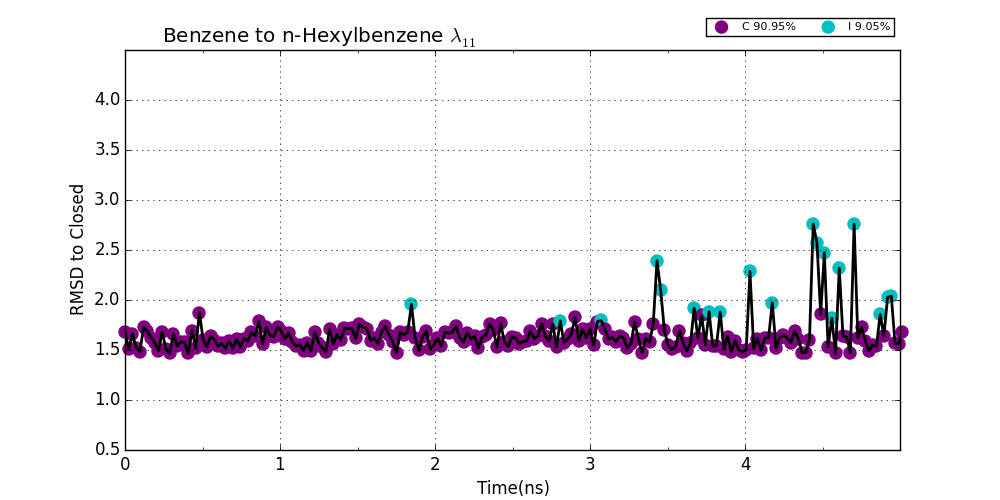
\includegraphics[trim={1.5cm 0 2cm 0.25cm}, clip, width=\textwidth,height=8cm]{VMDscripts/c_opls3_1/plots/0-5ns/RMSD-replica11.png}}
   \caption{Closed - Benzene to n-Hexylbenzene 0-5ns RMSD Replica11}
   \label{fig:c_opls3_1/RMSD-replica11}
\end{figure}

\begin{figure}[!h]
   \frame{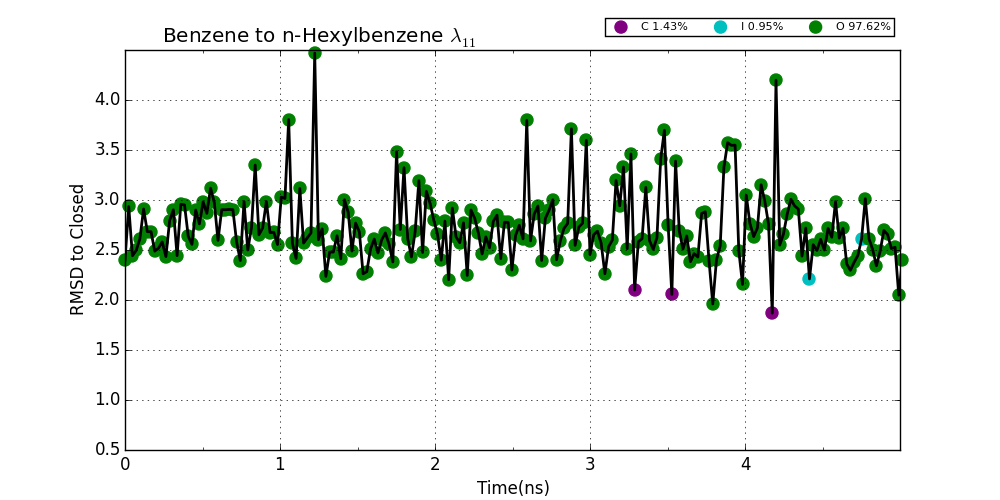
\includegraphics[trim={1.5cm 0 2cm 0.25cm}, clip, width=\textwidth,height=8cm]{VMDscripts/o_opls3_1/plots/0-5ns/RMSD-replica11.png}}
   \caption{Open - Benzene to n-Hexylbenzene 0-5ns RMSD Replica11}
   \label{fig:o_opls3_1/RMSD-replica11}
\end{figure}

\begin{figure}[!h]
   \frame{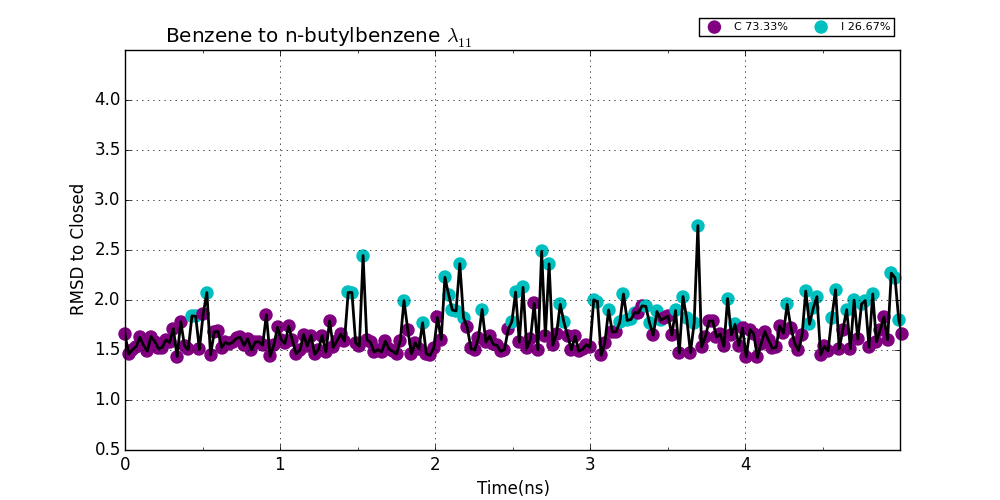
\includegraphics[trim={1.5cm 0 2cm 0.25cm}, clip, width=\textwidth,height=8cm]{VMDscripts/c_exp_opls3_11/plots/0-5ns/RMSD-replica11.png}}
   \caption{Closed - Benzene to n-butylbenzene 0-5ns RMSD Replica11}
   \label{fig:c_exp_opls3_11/RMSD-replica11}
\end{figure}

\begin{figure}[!h]
   \frame{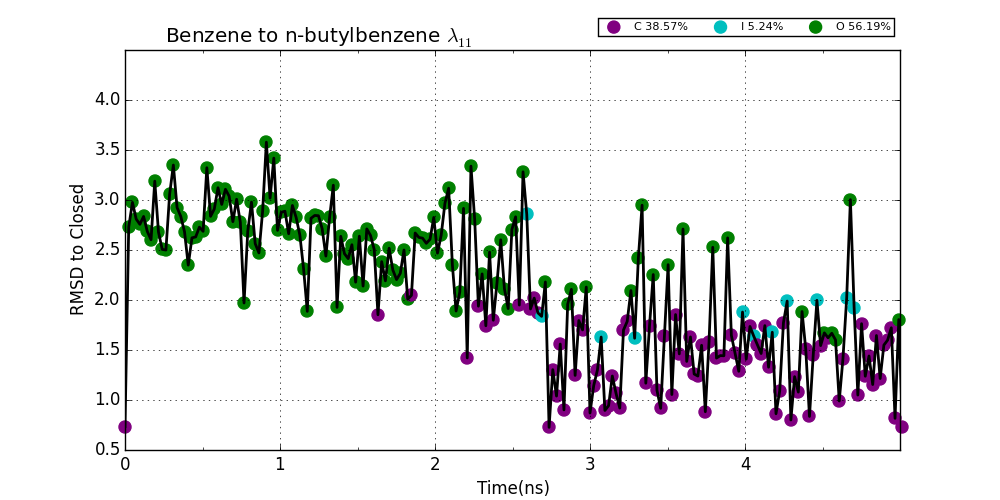
\includegraphics[trim={1.5cm 0 2cm 0.25cm}, clip, width=\textwidth,height=8cm]{VMDscripts/o_exp_opls3_24/plots/0-5ns/RMSD-replica11.png}}
   \caption{Open - Benzene to n-butylbenzene 0-5ns RMSD Replica11}
   \label{fig:o_exp_opls3_24/RMSD-replica11}
\end{figure}

\begin{figure}[!ht]
   \frame{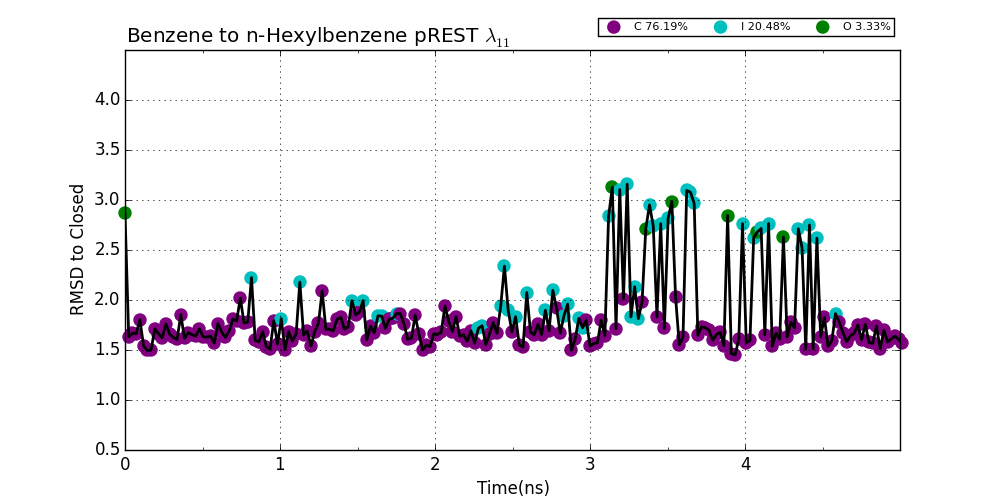
\includegraphics[trim={1.5cm 0 2cm 0.25cm}, clip, width=\textwidth,height=8cm]{VMDscripts/c_opls3_rest1_extend_1e/plots/0-5ns/RMSD-replica11.png}}
   \caption{Closed - Benzene to n-Hexylbenzene 0-5ns RMSD Replica11 pREST}
   \label{fig:c_opls3_rest1_1/RMSD-replica11}
\end{figure}

\begin{figure}[!ht]
   \frame{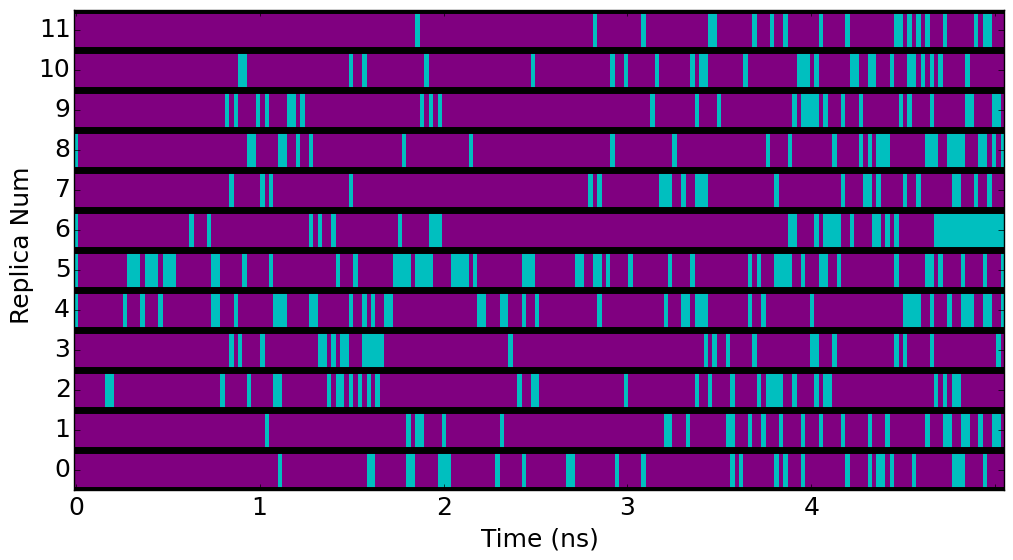
\includegraphics[trim={1.5cm 0 2cm 0.25cm}, clip, width=\textwidth,height=8cm]{VMDscripts/c_opls3_1/plots/colormap/cmap-0-5ns.png}}
   \caption{Closed - Benzene to n-Hexylbenzene 0-5ns Colormap}
   \label{fig:c_opls3_1/colormap}
\end{figure}

\begin{figure}[!ht]
   \frame{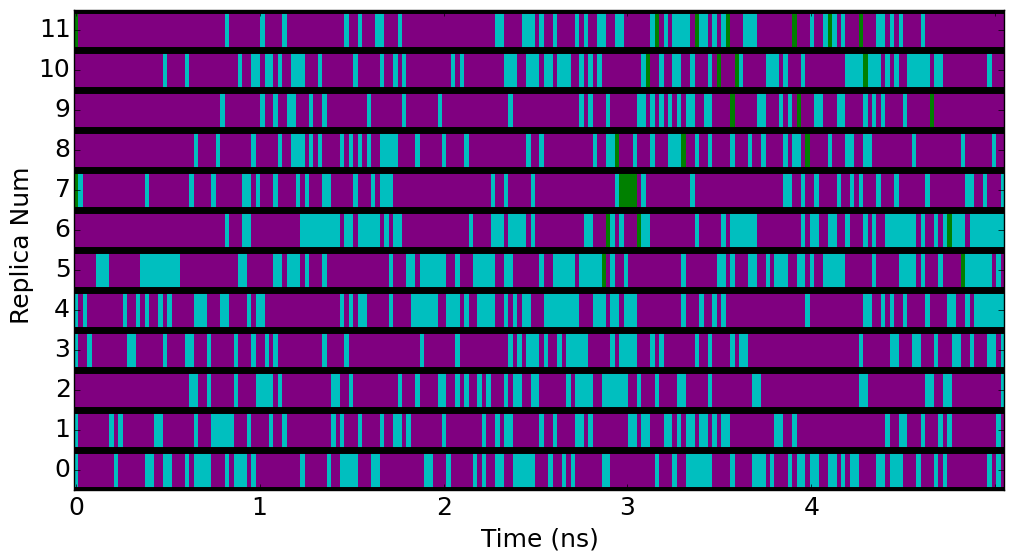
\includegraphics[trim={1.5cm 0 2cm 0.25cm}, clip, width=\textwidth,height=8cm]{VMDscripts/c_opls3_rest1_extend_1e/plots/colormap/cmap-0-5ns.png}}
   \caption{Closed - Benzene to n-Hexylbenzene 0-5ns Colormap pREST}
   \label{fig:c_opls3_rest1_1/colormap}
\end{figure}

\begin{figure}[!ht]
   \frame{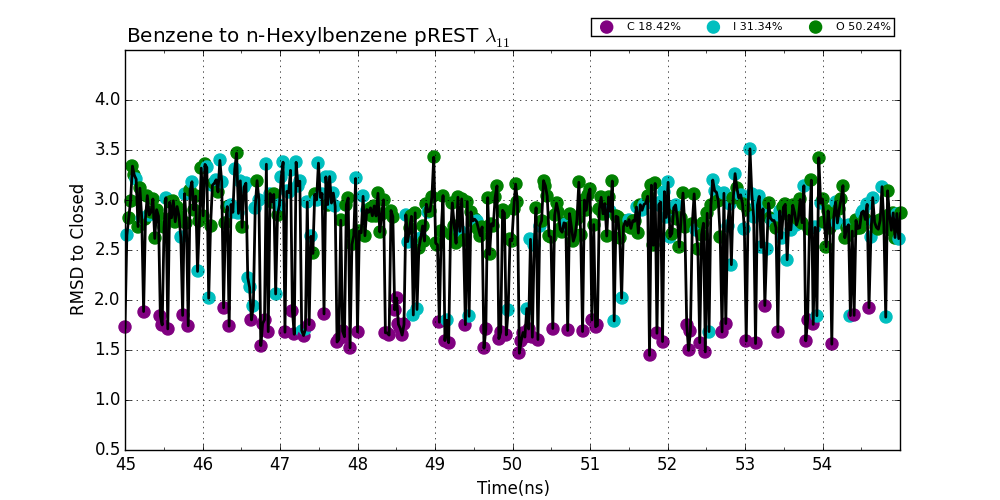
\includegraphics[trim={1.5cm 0 2cm 0.25cm}, clip, width=\textwidth,height=8cm]{VMDscripts/c_opls3_rest1_extend_1e/plots/45-55ns/RMSD-replica11.png}}
   \caption{Closed - Benzene to n-Hexylbenzene 45-55ns RMSD Replica11 pREST}
   \label{fig:c_opls3_rest1_1/45-55ns/RMSD-replica11}
\end{figure}

\begin{figure}[!ht]
   \frame{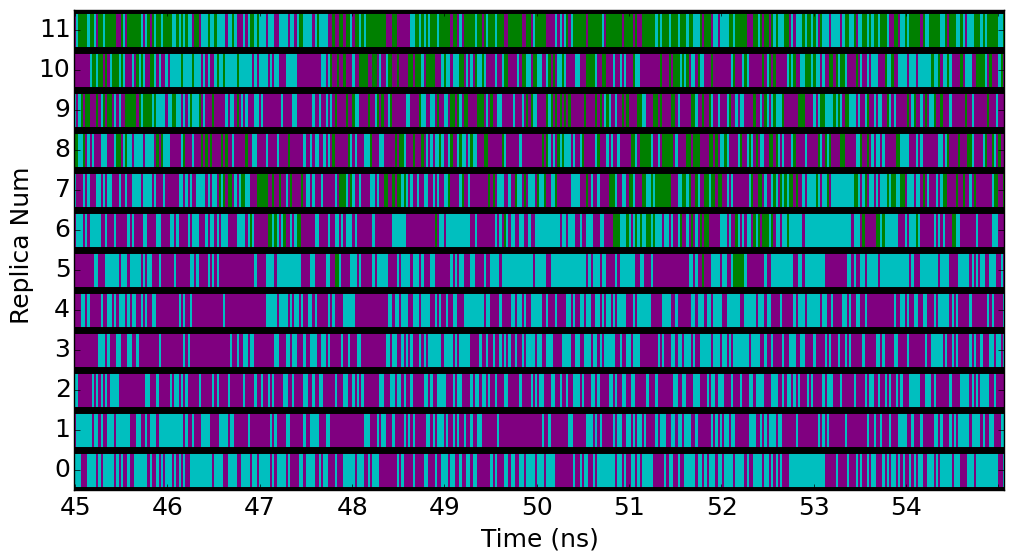
\includegraphics[trim={1.5cm 0 2cm 0.25cm}, clip, width=\textwidth,height=8cm]{VMDscripts/c_opls3_rest1_extend_1e/plots/colormap/cmap-45-55ns.png}}
   \caption{Closed - Benzene to n-Hexylbenzene 45-55ns Colormap pREST}
   \label{fig:c_opls3_rest1_1/cmap-45-55ns}
\end{figure}

\clearpage

\section{Tables}
\begin{table}[!htb]
\centering
\caption{Loop Occupancies \cite{Merski2015}}
\label{tbl:loop-occ}
\begin{tabular}{|c|c|c|c|}
\hline
\textbf{Ligand}                                                 & \textbf{C} & \textbf{I} & \textbf{O} \\ \hline
\cellcolor[HTML]{800080} benzene          & \cellcolor[HTML]{C0C0C0}0.9        & -          & -          \\ \hline
\cellcolor[HTML]{800080} toluene          & \cellcolor[HTML]{C0C0C0}0.8        & 0.2        & -          \\ \hline
\cellcolor[HTML]{800080} ethylbenzene     & \cellcolor[HTML]{C0C0C0}0.5        & 0.5        & -          \\ \hline
\cellcolor[HTML]{800080} n-propylbenzene  & \cellcolor[HTML]{C0C0C0}0.6        & 0.4        & -          \\ \hline
\cellcolor[HTML]{00FFFF} sec-butylbenzene & 0.4        & \cellcolor[HTML]{C0C0C0}0.6        & -          \\ \hline
\cellcolor[HTML]{00FFFF} n-butylbenzene   & 0.1        & \cellcolor[HTML]{C0C0C0}0.6        & 0.3        \\ \hline
\cellcolor[HTML]{008000} n-pentylbenzene  & 0.3        &    -        & \cellcolor[HTML]{C0C0C0}0.7        \\ \hline
\cellcolor[HTML]{008000} n-hexylbenzene   & 0.3        &    -       & \cellcolor[HTML]{C0C0C0}0.7        \\ \hline
\end{tabular}
\end{table}

\begin{table}[!htb]
\centering
\caption{Ligand Binding Affinities}
\label{tbl:lig-aff}
\begin{tabular}{|c|c|c|c|}
\hline
\textit{\textbf{PDB}} & \textbf{Ligand}                          & \boldmath$\Delta G_{exp}$                                            & \textbf{Error} \\ \hline
\textit{4W52}         & \cellcolor[HTML]{800080}benzene          & -5.19                                                                & 0.16           \\ \hline
\textit{4W53}         & \cellcolor[HTML]{800080}toluene          & -5.52                                                                & 0.04           \\ \hline
\textit{4W54}         & \cellcolor[HTML]{800080}ethylbenzene     & -5.76                                                                & 0.07           \\ \hline
\textit{4W55}         & \cellcolor[HTML]{800080}n-propylbenzene  & -6.55                                                                & 0.02           \\ \hline
\textit{4W56}         & \cellcolor[HTML]{00FFFF}sec-butylbenzene & N/A                                                                  & -              \\ \hline
\textit{4W57}         & \cellcolor[HTML]{00FFFF}n-butylbenezene  & -6.70                                                                & 0.02           \\ \hline
\textit{4W58}         & \cellcolor[HTML]{008000}n-pentylbenzene  & N/A                                                                  & -              \\ \hline
\textit{4W59}         & \cellcolor[HTML]{008000}n-hexylbenzene   & N/A                                                                  & -              \\ \hline
\end{tabular}
\end{table}

\begin{table}[!htb]
\centering
\caption{Closed-Intermediate Transformations}
\label{tbl:C-I}
\begin{tabular}{|c|c|c|l|c|l|c|}
\hline
\textbf{Ligand 1}                       & \textbf{Ligand 2}                        & {\color[HTML]{800080} \textbf{Closed}} & {\color[HTML]{800080} \textit{Err}} & {\color[HTML]{008000} \textbf{Open}} & {\color[HTML]{008000} \textit{Err}} & \textbf{C-O Diff}            \\ \hline
\cellcolor[HTML]{800080}benzene         & \cellcolor[HTML]{00FFFF}n-butylbenzene   & 0.58                                   & \textit{0.07}                       & -0.59                                & \textit{0.09}                       & \cellcolor[HTML]{FFCCC9}1.17 \\ \hline
\cellcolor[HTML]{800080}toluene         & \cellcolor[HTML]{00FFFF}n-butylbenzene   & -0.28                                  & \textit{0.06}                       & -1.27                                & \textit{0.09}                       & \cellcolor[HTML]{9AFF99}0.99 \\ \hline
\cellcolor[HTML]{800080}ethylbenzene    & \cellcolor[HTML]{00FFFF}n-butylbenzene   & 0.24                                   & \textit{0.07}                       & -0.23                                & \textit{0.07}                       & \cellcolor[HTML]{9AFF99}0.47 \\ \hline
\cellcolor[HTML]{800080}n-propylbenzene & \cellcolor[HTML]{00FFFF}n-butylbenzene   & 0.99                                   & \textit{0.06}                       & 0.63                                 & \textit{0.04}                       & \cellcolor[HTML]{9AFF99}0.36 \\ \hline
\cellcolor[HTML]{800080}benzene         & \cellcolor[HTML]{00FFFF}sec-butylbenzene & 2.36                                   & \textit{0.09}                       & 2.14                                 & \textit{0.11}                       & \cellcolor[HTML]{9AFF99}0.22 \\ \hline
\cellcolor[HTML]{800080}toluene         & \cellcolor[HTML]{00FFFF}sec-butylbenzene & 1.47                                   & \textit{0.07}                       & 1.14                                 & \textit{0.09}                       & \cellcolor[HTML]{9AFF99}0.33 \\ \hline
\cellcolor[HTML]{800080}ethylbenzene    & \cellcolor[HTML]{00FFFF}sec-butylbenzene & 1.90                                   & \textit{0.08}                       & 1.77                                 & \textit{0.07}                       & \cellcolor[HTML]{9AFF99}0.13 \\ \hline
\cellcolor[HTML]{800080}n-propylbenzene & \cellcolor[HTML]{00FFFF}sec-butylbenzene & 2.86                                   & \textit{0.06}                       & 2.67                                 & \textit{0.05}                       & \cellcolor[HTML]{9AFF99}0.19 \\ \hline
\end{tabular}
\end{table}

\begin{table}[!htb]
\centering
\caption{Closed-Intermediate Transformations pREST}
\label{tbl:C-I_pREST}
\begin{tabular}{|c|c|c|l|c|l|c|}
\hline
\textbf{Ligand 1}                       & \textbf{Ligand 2}                        & {\color[HTML]{800080} \textbf{Closed}} & {\color[HTML]{800080} \textit{Err}} & {\color[HTML]{008000} \textbf{Open}} & {\color[HTML]{008000} \textit{Err}} & \textbf{C-O Diff}            \\ \hline
\cellcolor[HTML]{800080}benzene         & \cellcolor[HTML]{00FFFF}n-butylbenzene   & -0.10                                   & \textit{0.11}                       & -0.72                                & \textit{0.12}                       & \cellcolor[HTML]{FFCCC9}0.62 \\ \hline
\cellcolor[HTML]{800080}toluene         & \cellcolor[HTML]{00FFFF}n-butylbenzene   & 0.90                                  & \textit{0.09}                       & -0.36                                & \textit{0.09}                       & \cellcolor[HTML]{9AFF99}1.26 \\ \hline
\cellcolor[HTML]{800080}ethylbenzene    & \cellcolor[HTML]{00FFFF}n-butylbenzene   & -0.20                                   & \textit{0.09}                       & -0.43                                & \textit{0.08}                       & \cellcolor[HTML]{9AFF99}0.23 \\ \hline
\cellcolor[HTML]{800080}n-propylbenzene & \cellcolor[HTML]{00FFFF}n-butylbenzene   & 1.00                                  & \textit{0.07}                       & 0.49                                 & \textit{0.06}                       & \cellcolor[HTML]{9AFF99}0.51 \\ \hline
\cellcolor[HTML]{800080}benzene         & \cellcolor[HTML]{00FFFF}sec-butylbenzene & 0.45                                   & \textit{0.08}                       & 1.34                                 & \textit{0.12}                       & \cellcolor[HTML]{9AFF99}0.89 \\ \hline
\cellcolor[HTML]{800080}toluene         & \cellcolor[HTML]{00FFFF}sec-butylbenzene & 0.60                                   & \textit{0.12}                       & 0.60                                 & \textit{0.10}                       & \cellcolor[HTML]{9AFF99}0.0 \\ \hline
\cellcolor[HTML]{800080}ethylbenzene    & \cellcolor[HTML]{00FFFF}sec-butylbenzene & 1.09                                   & \textit{0.10}                       & 1.69                                 & \textit{0.09}                       & \cellcolor[HTML]{9AFF99}0.60 \\ \hline
\cellcolor[HTML]{800080}n-propylbenzene & \cellcolor[HTML]{00FFFF}sec-butylbenzene & 1.88                                   & \textit{0.07}                       & 3.05                                 & \textit{0.08}                       & \cellcolor[HTML]{9AFF99}1.17 \\ \hline
\end{tabular}
\end{table}

\begin{table}[!htb]
\centering
\caption{Closed-Intermediate Transformations pREST 15-25ns}
\label{tbl:C-I_pRESText}
\begin{tabular}{|c|c|c|l|c|l|c|}
\hline
\textbf{Ligand 1}                       & \textbf{Ligand 2}                        & {\color[HTML]{800080} \textbf{Closed}} & {\color[HTML]{800080} \textit{Err}} & {\color[HTML]{008000} \textbf{Open}} & {\color[HTML]{008000} \textit{Err}} & \textbf{C-O Diff}            \\ \hline
\cellcolor[HTML]{800080}benzene         & \cellcolor[HTML]{00FFFF}n-butylbenzene   & -1.15                                   & \textit{0.09}                       & -0.72                                & \textit{0.12}                       & \cellcolor[HTML]{FFCCC9}0.43 \\ \hline
\cellcolor[HTML]{800080}toluene         & \cellcolor[HTML]{00FFFF}n-butylbenzene   & -0.52                                  & \textit{0.09}                       & -0.36                                & \textit{0.09}                       & \cellcolor[HTML]{9AFF99}0.16 \\ \hline
\cellcolor[HTML]{800080}ethylbenzene    & \cellcolor[HTML]{00FFFF}n-butylbenzene   & -0.20                                   & \textit{0.09}                       & -0.43                                & \textit{0.08}                       & \cellcolor[HTML]{9AFF99}0.23 \\ \hline
\cellcolor[HTML]{800080}n-propylbenzene & \cellcolor[HTML]{00FFFF}n-butylbenzene   & 0.53                                  & \textit{0.07}                       & 0.49                                 & \textit{0.06}                       & \cellcolor[HTML]{9AFF99}0.04 \\ \hline
\cellcolor[HTML]{800080}benzene         & \cellcolor[HTML]{00FFFF}sec-butylbenzene & 0.45                                   & \textit{0.08}                       & 1.34                                 & \textit{0.12}                       & \cellcolor[HTML]{9AFF99}0.89 \\ \hline
\cellcolor[HTML]{800080}toluene         & \cellcolor[HTML]{00FFFF}sec-butylbenzene & 0.60                                   & \textit{0.12}                       & 0.60                                 & \textit{0.10}                       & \cellcolor[HTML]{9AFF99}0.0 \\ \hline
\cellcolor[HTML]{800080}ethylbenzene    & \cellcolor[HTML]{00FFFF}sec-butylbenzene & 1.09                                   & \textit{0.10}                       & 1.69                                 & \textit{0.09}                       & \cellcolor[HTML]{9AFF99}0.60 \\ \hline
\cellcolor[HTML]{800080}n-propylbenzene & \cellcolor[HTML]{00FFFF}sec-butylbenzene & 1.88                                   & \textit{0.07}                       & 1.84                                 & \textit{0.06}                       & \cellcolor[HTML]{9AFF99}0.04 \\ \hline
\end{tabular}
\end{table}


\begin{table}[!htb]
\centering
\caption{Closed-Open Transformations}
\label{tbl:C-O}
\begin{tabular}{|c|c|c|l|c|l|c|}
\hline
\textbf{Ligand 1}                       & \textbf{Ligand 2}                       & {\color[HTML]{800080} \textbf{Closed}} & {\color[HTML]{800080} \textit{Err}} & {\color[HTML]{008000} \textbf{Open}} & {\color[HTML]{008000} \textit{Err}} & \textbf{C-O Diff}            \\ \hline
\cellcolor[HTML]{800080}benzene         & \cellcolor[HTML]{008000}n-pentylbenzene & 2.36                                   & \textit{0.12}                       & -1.33                                & \textit{0.11}                       & \cellcolor[HTML]{FFCCC9}3.69 \\ \hline
\cellcolor[HTML]{800080}toluene         & \cellcolor[HTML]{008000}n-pentylbenzene & 1.77                                   & \textit{0.09}                       & 0.34                                 & \textit{0.10}                       & \cellcolor[HTML]{FFCCC9}1.43 \\ \hline
\cellcolor[HTML]{800080}ethylbenzene    & \cellcolor[HTML]{008000}n-pentylbenzene & 2.45                                   & \textit{0.08}                       & 0.46                                 & \textit{0.09}                       & \cellcolor[HTML]{FFCCC9}1.99 \\ \hline
\cellcolor[HTML]{800080}n-propylbenzene & \cellcolor[HTML]{008000}n-pentylbenzene & 3.46                                   & \textit{0.08}                       & -0.22                                & \textit{0.08}                       & \cellcolor[HTML]{FFCCC9}3.68 \\ \hline
\cellcolor[HTML]{800080}benzene         & \cellcolor[HTML]{008000}n-hexylbenzene  & 4.13                                   & \textit{0.16}                       & -0.61                                & \textit{0.15}                       & \cellcolor[HTML]{FFCCC9}4.74 \\ \hline
\cellcolor[HTML]{800080}toluene         & \cellcolor[HTML]{008000}n-hexylbenzene  & 2.90                                   & \textit{0.14}                       & -1.63                                & \textit{0.08}                       & \cellcolor[HTML]{FFCCC9}4.53 \\ \hline
\cellcolor[HTML]{800080}ethylbenzene    & \cellcolor[HTML]{008000}n-hexylbenzene  & 3.63                                   & \textit{0.11}                       & -0.76                                & \textit{0.09}                       & \cellcolor[HTML]{FFCCC9}4.39 \\ \hline
\cellcolor[HTML]{800080}n-propylbenzene & \cellcolor[HTML]{008000}n-hexylbenzene  & 5.85                                   & \textit{0.10}                       & 0.13                                 & \textit{0.06}                       & \cellcolor[HTML]{FFCCC9}5.72 \\ \hline
\end{tabular}

  \textsuperscript{\emph{a}} Some text;
  \textsuperscript{\emph{b}} Some more text.
\end{table}

\begin{table}[!htb]
\centering
\caption{Closed-Open Transformations pREST}
\label{tbl:C-O_pREST}
\begin{tabular}{|c|c|c|l|c|l|c|}
\hline
\textbf{Ligand 1}                       & \textbf{Ligand 2}                       & {\color[HTML]{800080} \textbf{Closed}} & {\color[HTML]{800080} \textit{Err}} & {\color[HTML]{008000} \textbf{Open}} & {\color[HTML]{008000} \textit{Err}} & \textbf{C-O Diff}            \\ \hline
\cellcolor[HTML]{800080}benzene         & \cellcolor[HTML]{008000}n-pentylbenzene & 1.45                                   & \textit{0.13}                       & 0.15                                & \textit{0.10}                       & \cellcolor[HTML]{FFCCC9}1.30 \\ \hline
\cellcolor[HTML]{800080}toluene         & \cellcolor[HTML]{008000}n-pentylbenzene & 1.40                                   & \textit{0.13}                       & 0.82                                 & \textit{0.11}                       & \cellcolor[HTML]{FFCCC9}0.58 \\ \hline
\cellcolor[HTML]{800080}ethylbenzene    & \cellcolor[HTML]{008000}n-pentylbenzene & 2.89                                   & \textit{0.10}                       & 1.32                                 & \textit{0.10}                       & \cellcolor[HTML]{FFCCC9}1.57 \\ \hline
\cellcolor[HTML]{800080}n-propylbenzene & \cellcolor[HTML]{008000}n-pentylbenzene & 4.40                                   & \textit{0.12}                       & 1.06                                & \textit{0.09}                       & \cellcolor[HTML]{FFCCC9}3.34 \\ \hline
\cellcolor[HTML]{800080}benzene         & \cellcolor[HTML]{008000}n-hexylbenzene  & 2.74                                   & \textit{0.19}                       & 1.37                                & \textit{0.13}                       & \cellcolor[HTML]{FFCCC9}1.37 \\ \hline
\cellcolor[HTML]{800080}toluene         & \cellcolor[HTML]{008000}n-hexylbenzene  & 3.21                                   & \textit{0.15}                       & -1.08                                & \textit{0.09}                       & \cellcolor[HTML]{FFCCC9}4.29 \\ \hline
\cellcolor[HTML]{800080}ethylbenzene    & \cellcolor[HTML]{008000}n-hexylbenzene  & 3.39                                   & \textit{0.11}                       & -0.14                                & \textit{0.10}                       & \cellcolor[HTML]{FFCCC9}3.53 \\ \hline
\cellcolor[HTML]{800080}n-propylbenzene & \cellcolor[HTML]{008000}n-hexylbenzene  & 4.93                                   & \textit{0.12}                       & 1.28                                 & \textit{0.10}                       & \cellcolor[HTML]{FFCCC9}3.65 \\ \hline
\end{tabular}

  \textsuperscript{\emph{a}} Some text;
  \textsuperscript{\emph{b}} Some more text.
\end{table}

\begin{table}[!htb]
\centering
\caption{Closed-Open Transformations pREST 40-55ns}
\label{tbl:C-O_pREST-40-55ns}
\begin{tabular}{|c|c|c|l|c|l|c|}
\hline
\textbf{Ligand 1}                       & \textbf{Ligand 2}                       & {\color[HTML]{800080} \textbf{Closed}} & {\color[HTML]{800080} \textit{Err}} & {\color[HTML]{008000} \textbf{Open}} & {\color[HTML]{008000} \textit{Err}} & \textbf{C-O Diff}            \\ \hline
\cellcolor[HTML]{800080}benzene         & \cellcolor[HTML]{008000}n-pentylbenzene & 1.86                                   & \textit{0.06}                       & 1.50                                & \textit{0.06}                       & \cellcolor[HTML]{FFCCC9}0.36 \\ \hline
\cellcolor[HTML]{800080}toluene         & \cellcolor[HTML]{008000}n-pentylbenzene & 1.03                                   & \textit{0.06}                       & 0.71                                 & \textit{0.06}                       & \cellcolor[HTML]{FFCCC9}0.32 \\ \hline
\cellcolor[HTML]{800080}ethylbenzene    & \cellcolor[HTML]{008000}n-pentylbenzene & 1.69                                   & \textit{0.06}                       & 1.60                                 & \textit{0.06}                       & \cellcolor[HTML]{FFCCC9}0.09 \\ \hline
\cellcolor[HTML]{800080}n-propylbenzene & \cellcolor[HTML]{008000}n-pentylbenzene & 3.43                                   & \textit{0.04}                       & 2.44                                & \textit{0.04}                       & \cellcolor[HTML]{FFCCC9}0.99 \\ \hline
\cellcolor[HTML]{800080}benzene         & \cellcolor[HTML]{008000}n-hexylbenzene  & 2.14                                   & \textit{0.08}                       & 1.41                                & \textit{0.07}                       & \cellcolor[HTML]{FFCCC9}0.73 \\ \hline
\cellcolor[HTML]{800080}toluene         & \cellcolor[HTML]{008000}n-hexylbenzene  & 0.33                                   & \textit{0.08}                       & 1.16                                & \textit{0.06}                       & \cellcolor[HTML]{FFCCC9}0.84 \\ \hline
\cellcolor[HTML]{800080}ethylbenzene    & \cellcolor[HTML]{008000}n-hexylbenzene  & 1.97                                   & \textit{0.07}                       & 2.39                                & \textit{0.06}                       & \cellcolor[HTML]{FFCCC9}0.42 \\ \hline
\cellcolor[HTML]{800080}n-propylbenzene & \cellcolor[HTML]{008000}n-hexylbenzene  & 3.49                                   & \textit{0.06}                       & 3.44                                 & \textit{0.05}                       & \cellcolor[HTML]{FFCCC9}0.05 \\ \hline
\end{tabular}

  \textsuperscript{\emph{a}} Some text;
  \textsuperscript{\emph{b}} Some more text.
\end{table}

\begin{table}[!htb]
\centering
\caption{Closed to n-butylbenzene Transformations (Closed Protein)}
\label{tbl:C-nbutyl_closed}
\begin{tabular}{|c|c|c|l|c|}
\hline
\textbf{Ligand 1}                       & \textbf{Ligand 2}                      & {\color[HTML]{800080} \textbf{Closed}} & {\color[HTML]{800080} \textit{Err}} & \textbf{C-Exp Err}           \\ \hline
\cellcolor[HTML]{800080}benzene         & \cellcolor[HTML]{00FFFF}n-butylbenzene & 0.58                                   & \textit{0.07}                       & \cellcolor[HTML]{FFCCC9}2.09 \\ \hline
\cellcolor[HTML]{800080}toluene         & \cellcolor[HTML]{00FFFF}n-butylbenzene & -0.28                                  & \textit{0.06}                       & \cellcolor[HTML]{9AFF99}0.90 \\ \hline
\cellcolor[HTML]{800080}ethylbenzene    & \cellcolor[HTML]{00FFFF}n-butylbenzene & 0.24                                   & \textit{0.07}                       & \cellcolor[HTML]{FFCCC9}1.18 \\ \hline
\cellcolor[HTML]{800080}n-propylbenzene & \cellcolor[HTML]{00FFFF}n-butylbenzene & 0.99                                   & \textit{0.06}                       & \cellcolor[HTML]{FFCCC9}1.14 \\ \hline
\end{tabular}
\end{table}

\begin{table}[!htb]
\centering
\caption{Closed to n-butylbenzene Transformations (Open Protein)}
\label{tbl:C-nbutyl_open}
\begin{tabular}{|c|c|c|l|c|}
\hline
\textbf{Ligand 1}                       & \textbf{Ligand 2}                      & {\color[HTML]{008000} \textbf{Open}} & {\color[HTML]{008000} \textit{Err}} & \textbf{O-Exp Err}           \\ \hline
\cellcolor[HTML]{800080}benzene         & \cellcolor[HTML]{00FFFF}n-butylbenzene & -0.59                                & \textit{0.09}                       & \cellcolor[HTML]{9AFF99}0.92 \\ \hline
\cellcolor[HTML]{800080}toluene         & \cellcolor[HTML]{00FFFF}n-butylbenzene & -1.27                                & \textit{0.09}                       & \cellcolor[HTML]{9AFF99}0.09 \\ \hline
\cellcolor[HTML]{800080}ethylbenzene    & \cellcolor[HTML]{00FFFF}n-butylbenzene & -0.23                                & \textit{0.07}                       & \cellcolor[HTML]{9AFF99}0.71 \\ \hline
\cellcolor[HTML]{800080}n-propylbenzene & \cellcolor[HTML]{00FFFF}n-butylbenzene & 0.63                                 & \textit{0.04}                       & \cellcolor[HTML]{9AFF99}0.78 \\ \hline
\end{tabular}
\end{table}

\clearpage

\bibliography{references}
\end{document}
